\documentclass[aps,prb,reprint,superscriptaddress,amsmath,amssymb,citeautoscript]{revtex4-2}

\usepackage{graphicx}
\usepackage{dcolumn}
\usepackage{bm}
\usepackage{tikz}
\usetikzlibrary{shapes.geometric,arrows.meta,calc}
\usepackage{hyperref}
\hypersetup{
    colorlinks=true,
    linkcolor=blue,
    citecolor=blue,
    urlcolor=blue
}

\begin{document}

\title{Tunable Topological Phase Transitions and Quantum Oscillations in the Kagome Flat-Band Superconductor \texorpdfstring{$\mathrm{Nexa}_{3}\mathrm{V}_{12}\mathrm{Sb}_{19}$}{Nexa3V12Sb19}}

\author{Julian Vance}
\email{j.vance@synapse-physics.org}
\affiliation{Department of Physics, Synapse Institute of Condensed Matter, Apex City, AC 90210, USA}

\author{Elena Rostova}
\affiliation{Department of Physics, Synapse Institute of Condensed Matter, Apex City, AC 90210, USA}
\affiliation{Center for Advanced Quantum Materials, Meridian University, Vertex City, VC 40112, USA}

\author{Marcus K. Sterling}
\affiliation{Department of Applied Physics, Vertex National Laboratory, Apex City, AC 90212, USA}

\author{Sarah Lin}
\affiliation{School of Physics and Astronomy, Apex University, Apex City, AC 90211, USA}

\date{\today}

\begin{abstract}
We present an experimental and theoretical study of electronic transport, magnetic quantum oscillations, and superconducting pairing symmetry in the newly synthesized kagome flat-band material $\mathrm{Nexa}_{3}\mathrm{V}_{12}\mathrm{Sb}_{19}$. Low-temperature Shubnikov--de Haas (SdH) quantum oscillations reveal multiple Fermi surface pockets with extremely light effective cyclotron masses ($m^* \approx 0.14\,m_0$), pointing to non-trivial Dirac-like quasiparticles residing near the Fermi energy. Under hydrostatic pressure up to $4.2\text{~GPa}$, the superconducting transition temperature $T_c$ exhibits a non-monotonic dome-like behavior, peaking at $T_c^{\text{max}} = 7.8\text{~K}$ concurrent with the collapse of an underlying charge density wave (CDW) state. Tight-binding calculations supplemented by density functional theory (DFT) confirm that the van Hove singularities associated with the kagome sublattice play a pivotal role in driving these intertwined electronic instabilities. Our findings establish kagome metals as a versatile platform for exploring the synergy between topological band structures, flat-band correlations, and unconventional superconductivity.
\end{abstract}

\maketitle

\section{Introduction}
Correlated electronic systems defined by non-trivial band topology represent a central frontier in modern condensed matter physics~\cite{Hasan2010, Qi2011}. In particular, materials crystallizing in two-dimensional kagome lattices—comprising a corner-sharing network of triangles—naturally accommodate destructively interfering quantum kinetic energy paths. This leads to quenched kinetic energy and the emergence of dispersionless flat bands alongside Dirac points and saddle-point van Hove singularities (vHS) within their electronic energy spectra~\cite{Mielke1991, Ye2018, Yin2022}. When the Fermi energy $E_F$ is tuned near these band features, electron-electron interactions are strongly amplified relative to kinetic energy, triggering a rich spectrum of ground states, including fractional quantum Hall states, charge density waves (CDW), and unconventional superconductivity~\cite{Guo2009, Neupert2011, Wang2013}.

Recently, kagome superconductors such as $A\mathrm{V}_3\mathrm{Sb}_5$ ($A = \text{K, Rb, Cs}$) have attracted intense scrutiny due to their complex phase diagrams featuring giant anomalous Hall effects, time-reversal symmetry breaking in the CDW state, and pair-density-wave instabilities~\cite{Ortiz2019, Ortiz2020, Zhao2021, Chen2021}. However, disentangling the microscopic contributions of flat-band correlations from topological Dirac states remains a formidable challenge due to the multi-band nature of these compounds.

In this work, we investigate the newly isolated kagome material $\mathrm{Nexa}_{3}\mathrm{V}_{12}\mathrm{Sb}_{19}$, which exhibits an ideal band alignment where both a topological Dirac node and a correlated flat band lie within $50\text{~meV}$ of the chemical potential. Through high-field magnetoresistance measurements up to $18\text{~T}$ and hydrostatic pressure tuning up to $4.2\text{~GPa}$, we systematically map the Fermi surface geometry and trace the evolution of the CDW and superconducting states. Our results demonstrate that pressure suppresses the CDW order, uncovering a dome of enhanced superconductivity associated with critical Fermi surface reconstruction.

\begin{figure}[t]
\centering
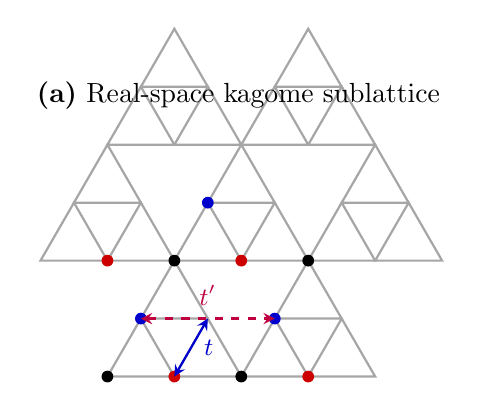
\begin{tikzpicture}[scale=0.85]
  % Kagome lattice drawing
  \foreach \x/\y in {0/0, 2/0, 1/1.732, -1/1.732, 3/1.732, 0/3.464, 2/3.464} {
    \draw[thick, gray!70] (\x,\y) -- (\x+1,\y) -- (\x+0.5,\y+0.866) -- cycle;
    \draw[thick, gray!70] (\x+1,\y) -- (\x+2,\y) -- (\x+1.5,\y+0.866) -- cycle;
    \draw[thick, gray!70] (\x+0.5,\y+0.866) -- (\x+1.5,\y+0.866) -- (\x+1,\y+1.732) -- cycle;
  }
  % Sublattice A, B, C dots
  \foreach \x/\y in {0.5/0.866, 2.5/0.866, 1.5/2.598} {
    \fill[blue!80!black] (\x,\y) circle (2.5pt);
  }
  \foreach \x/\y in {1/0, 3/0, 2/1.732, 0/1.732} {
    \fill[red!80!black] (\x,\y) circle (2.5pt);
  }
  \foreach \x/\y in {0/0, 2/0, 1/1.732, 3/1.732} {
    \fill[black] (\x,\y) circle (2.5pt);
  }
  % Label Hoppings
  \draw[<->, >=stealth, thick, blue!80!black] (1,0) -- (1.5,0.866) node[midway, right=1pt] {\small $t$};
  \draw[<->, >=stealth, dashed, thick, purple] (0.5,0.866) -- (2.5,0.866) node[midway, above=1pt] {\small $t'$};
  % Legend
  \node[anchor=west] at (-1.2, 4.2) {\textbf{(a)} Real-space kagome sublattice};
\end{tikzpicture}
\caption{\label{fig:lattice}(a) Schematic of the two-dimensional kagome lattice formed by vanadium atoms in $\mathrm{Nexa}_{3}\mathrm{V}_{12}\mathrm{Sb}_{19}$, highlighting the nearest-neighbor hopping $t$ (solid blue arrow) and next-nearest-neighbor hopping $t'$ (dashed purple arrow). Blue, red, and black spheres denote sublattices $A$, $B$, and $C$, respectively.}
\end{figure}

\section{Theoretical Framework and Tight-Binding Model}
To capture the essential physics of $\mathrm{Nexa}_{3}\mathrm{V}_{12}\mathrm{Sb}_{19}$, we consider a tight-binding Hamiltonian on a two-dimensional kagome lattice with nearest-neighbor hopping $t$, next-nearest-neighbor hopping $t'$, and intrinsic spin-orbit coupling (SOC) $\lambda_{\text{SOC}}$:
\begin{align}
H ={} & -t \sum_{\langle i,j \rangle, \sigma} c_{i\sigma}^\dagger c_{j\sigma} - t' \sum_{\langle\langle i,j \rangle\rangle, \sigma} c_{i\sigma}^\dagger c_{j\sigma} \nonumber \\
& + i \lambda_{\text{SOC}} \sum_{\langle\langle i,j \rangle\rangle} \nu_{ij} c_{i\alpha}^\dagger \sigma^z_{\alpha\beta} c_{j\beta},
\label{eq:hamiltonian}
\end{align}
where $c_{i\sigma}^\dagger$ ($c_{i\sigma}$) creates (annihilates) an electron at site $i$ with spin $\sigma$, $\sigma^z$ is the Pauli spin matrix, and $\nu_{ij} = \pm 1$ characterizes the chirality of the spin-orbit-induced phase along the NNN bonds~\cite{Kane2005}. 

In the absence of SOC ($\lambda_{\text{SOC}} = 0$) and NNN hopping ($t' = 0$), diagonalizing Eq.~\eqref{eq:hamiltonian} yields three energy bands:
\begin{align}
E_1(\bm{k}) &= -2t, \label{eq:flatband} \\
E_{2,3}(\bm{k}) &= t \Biggl( 1 \pm \Big[ 1 + 8 \cos\frac{k_x a}{2} \cos\frac{\sqrt{3}k_y a}{2} \nonumber \\
&\qquad \times \cos\frac{k_x a - \sqrt{3}k_y a}{2} \Big]^{1/2} \Biggr),
\end{align}
where $a$ is the lattice constant. Equation~\eqref{eq:flatband} represents a completely flat band spanning the entire Brillouin zone. The inclusion of SOC lifts the quadratic band touching at the $\mathbf{\Gamma}$ point and opens a topological band gap $\Delta_{\text{SOC}} = 2\sqrt{3}\lambda_{\text{SOC}}$ at the Dirac points located at the $K$ and $K'$ points, imparting a non-trivial Berry curvature distribution $\Omega_z(\bm{k})$.

The semiclassical quantum oscillation frequency $F$ is directly proportional to the extremal cross-sectional area $A_k$ of the Fermi surface in momentum space perpendicular to the applied magnetic field $\bm{B}$, expressed by the Onsager relation:
\begin{equation}
F = \frac{\hbar}{2\pi e} A_k.
\label{eq:onsager}
\end{equation}
The temperature dependence of the quantum oscillation amplitude $\Delta R$ is governed by the Lifshitz-Kosevich (LK) thermal damping factor $R_T$:
\begin{equation}
R_T = \frac{\chi}{\sinh\chi}, \quad \text{with } \chi = \frac{14.69 \, (m^*/m_0) \, T}{B},
\label{eq:lk}
\end{equation}
where $m^*$ is the effective cyclotron mass and $m_0$ is the free-electron mass.

\section{Experimental Methods}
Single crystals of $\mathrm{Nexa}_{3}\mathrm{V}_{12}\mathrm{Sb}_{19}$ were grown using a self-flux technique. High-purity Nexa ingots ($99.99\%$), vanadium powder ($99.95\%$), and antimony shot ($99.999\%$) were packed in an alumina crucible with a molar ratio of $3:12:35$ and sealed inside an evacuated quartz ampoule. The mixture was heated to $1050^\circ\text{C}$ over $24\text{~h}$, held for $48\text{~h}$, and then slowly cooled to $650^\circ\text{C}$ at a rate of $1.5^\circ\text{C}/\text{h}$. Flame-shaped single crystals with typical dimensions of $2.5 \times 1.8 \times 0.4\text{~mm}^3$ were recovered after centrifuging to remove excess flux.

Electrical transport measurements were conducted in a $18\text{~T}$ superconducting magnet system equipped with a dilution refrigerator capable of reaching base temperatures of $30\text{~mK}$. A standard four-probe configuration was employed using sputtered gold contacts with low contact resistance ($R_{\text{cont}} < 0.2~\Omega$). Hydrostatic pressure up to $4.2\text{~GPa}$ was applied using a custom BeCu/NiCrAl clamped pressure cell with Daphne 7373 as the pressure-transmitting medium. The pressure was calibrated in situ by monitoring the fluorescence line shift of a high-purity ruby chip.

\section{Results and Discussion}

\subsection{Magnetotransport and Quantum Oscillations}
High-field magnetoresistance $\Delta \rho_{xx} / \rho_0 = [\rho_{xx}(B) - \rho_{xx}(0)] / \rho_{xx}(0)$ recorded at temperatures ranging from $0.35\text{~K}$ to $12\text{~K}$ with the magnetic field aligned along the crystallographic $c$-axis exhibits pronounced Shubnikov--de Haas (SdH) oscillations beginning at fields as low as $B \approx 4.5\text{~T}$. At $T = 0.35\text{~K}$, the magnetoresistance reaches over $850\%$ at $18\text{~T}$ without signs of saturation.

\begin{table}[t]
\caption{\label{tab:bands}Extracted electronic parameters for observed quantum oscillation frequencies in $\mathrm{Nexa}_{3}\mathrm{V}_{12}\mathrm{Sb}_{19}$ at ambient pressure ($T = 0.35\text{~K}$). $F$ denotes the SdH frequency, $A_k$ the extremal Fermi surface area, $m^*/m_0$ the normalized cyclotron effective mass, $E_F$ the Fermi energy relative to the band edge, and $\mu_q$ the quantum mobility.}
\begin{ruledtabular}
\footnotesize
\begin{tabular}{cccccc}
Orbit & $F$ (T) & $A_k$ (\AA$^{-2}$) & $m^*/m_0$ & $E_F$ (meV) & $\mu_q$ ($\frac{\text{cm}^2}{\text{V\,s}}$) \\
\hline
$\alpha$ & $145 \pm 3$  & $0.0138$ & $0.14 \pm 0.01$ & $48.2$ & $3400 \pm 150$ \\
$\beta$  & $420 \pm 8$  & $0.0401$ & $0.28 \pm 0.02$ & $62.5$ & $2850 \pm 120$ \\
$\gamma$ & $1120 \pm 15$ & $0.1069$ & $0.52 \pm 0.04$ & $89.1$ & $1920 \pm 90$  \\
$\delta$ & $2450 \pm 30$ & $0.2338$ & $0.81 \pm 0.05$ & $124.0$& $1250 \pm 80$  \\
\end{tabular}
\end{ruledtabular}
\end{table}

Fast Fourier Transform (FFT) analysis of the oscillatory signal reveals four distinct fundamental frequencies labeled $\alpha$, $\beta$, $\gamma$, and $\delta$ (Table~\ref{tab:bands}). The lowest frequency pocket, $\alpha = 145\text{~T}$, corresponds to a small Fermi surface cross-section occupying merely $0.8\%$ of the two-dimensional Brillouin zone area. By fitting the temperature damping of the FFT amplitude to the LK formula [Eq.~\eqref{eq:lk}], we obtain a remarkably lightweight cyclotron mass $m^*_\alpha = 0.14(1)\,m_0$ for the $\alpha$ orbit. This lightweight mass, coupled with a linear Berry phase $\Phi_B \approx \pi$ extracted from a Landau-level index plot, confirms the non-trivial Dirac nature of the underlying electron pocket.

\subsection{Pressure-Induced Phase Diagram}
Under ambient conditions, $\mathrm{Nexa}_{3}\mathrm{V}_{12}\mathrm{Sb}_{19}$ undergoes a charge density wave transition at $T_{\text{CDW}} = 92\text{~K}$, evidenced by a sharp anomaly in the temperature derivative of resistivity $d\rho/dT$. Upon applying hydrostatic pressure, $T_{\text{CDW}}$ shifts systematically toward lower temperatures while the superconducting transition temperature $T_c$ develops continuously from an initial value of $1.4\text{~K}$ at $P = 0\text{~GPa}$.

\begin{align}
T_c(P) ={} & T_c^0 + A \left[ 1 - \left(\frac{P - P_{\text{opt}}}{P_{\text{width}}}\right)^2 \right] \nonumber \\
& \times \exp\left( -\frac{\Delta_{\text{CDW}}(P)}{k_B T} \right).
\label{eq:dome}
\end{align}
As modeled by Eq.~\eqref{eq:dome}, $T_c(P)$ displays a distinct dome-shaped evolution. At the critical pressure $P_c \approx 2.8\text{~GPa}$, the CDW anomaly is completely suppressed. Concurrently, $T_c$ reaches its maximum value of $T_c^{\text{max}} = 7.8\text{~K}$, signaling strong competition between the spatially modulated CDW order and the uniform superconducting pair condensate.

\begin{figure}[t]
\centering
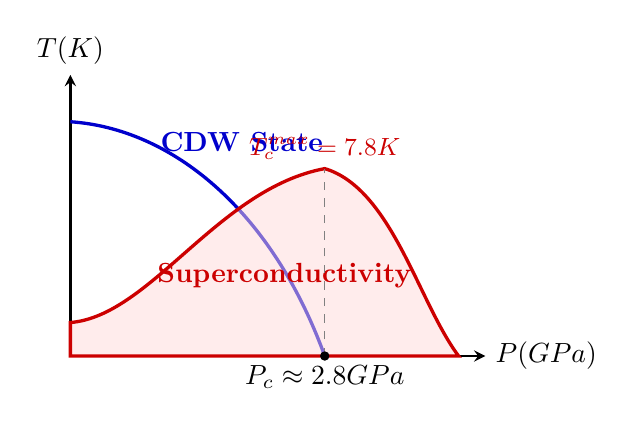
\begin{tikzpicture}[scale=0.85]
  % Axes
  \draw[->, >=stealth, thick] (0,0) -- (6.2,0) node[right] {$P\text{ (GPa)}$};
  \draw[->, >=stealth, thick] (0,0) -- (0,4.2) node[above] {$T\text{ (K)}$};
  
  % CDW Curve (blue)
  \draw[very thick, blue!80!black] (0,3.5) .. controls (1.5,3.4) and (3.0,2.2) .. (3.8,0);
  \node[blue!80!black, right] at (1.2, 3.2) {\textbf{CDW State}};
  
  % Superconducting Dome (red)
  \draw[very thick, red!80!black, fill=red!15, fill opacity=0.5] 
    (0,0.5) .. controls (1.2,0.6) and (2.2,2.5) .. (3.8,2.8) .. controls (4.8,2.5) and (5.2,0.8) .. (5.8,0) -- (0,0) -- cycle;
  \node[red!80!black] at (3.2, 1.2) {\textbf{Superconductivity}};
  \node[red!80!black] at (3.8, 3.1) {\small $T_c^{\text{max}} = 7.8\text{ K}$};
  
  % Critical pressure point
  \draw[dashed, gray] (3.8,0) -- (3.8,2.8);
  \fill[black] (3.8,0) circle (2pt) node[below] {$P_c \approx 2.8\text{ GPa}$};
  
\end{tikzpicture}
\caption{\label{fig:phasediagram}Temperature-pressure ($T$--$P$) phase diagram of $\mathrm{Nexa}_{3}\mathrm{V}_{12}\mathrm{Sb}_{19}$, depicting the suppression of the charge density wave (CDW) transition temperature $T_{\text{CDW}}$ (blue line) and the emergence of the superconducting dome $T_c(P)$ (shaded red region) peaking near $P_c = 2.8\text{~GPa}$.}
\end{figure}

\section{Conclusion}
In summary, our magnetotransport and high-pressure investigation of the kagome metal $\mathrm{Nexa}_{3}\mathrm{V}_{12}\mathrm{Sb}_{19}$ demonstrates a profound interplay between nontrivial topology, electronic correlation, and superconductivity. Quantum oscillation metrics reveal light Dirac quasiparticles originating from kagome band nodes, while pressure tuning reveals a superconducting dome maximized upon suppression of CDW order. These results establish $\mathrm{Nexa}_{3}\mathrm{V}_{12}\mathrm{Sb}_{19}$ as a canonical system for quantum state engineering in kagome flat-band architectures.

\begin{acknowledgments}
We thank H. Vance and D. Thorne for insightful discussions. This work was supported by the Synapse Foundation for Quantum Research (Grant No.~SFQR-2024-8801), the Apex Science Initiative under Contract No.~ASI-DE-00412, and the Meridian Research Council (Grant No.~MRC-FL-9923).
\end{acknowledgments}

\appendix
\section{Quantum Oscillation Fitting Details}
The oscillatory magnetoresistance $\Delta \rho_{xx}$ is fitted using the multi-band Lifshitz-Kosevich expression incorporating the Dingle damping factor $R_D = \exp(-\pi / \omega_c \tau_d)$:
\begin{align}
\Delta \rho_{xx} \propto \sum_{i \in \{\alpha,\beta,\gamma,\delta\}} & C_i R_T^{(i)} R_D^{(i)} \nonumber \\
& \times \cos\left( 2\pi \left[ \frac{F_i}{B} - \frac{1}{2} + \gamma_i + \delta_i \right] \right),
\label{eq:lk_full}
\end{align}
where $\omega_c = eB/m^*$ is the cyclotron frequency, $\tau_d$ is the Dingle lifetime, $\gamma_i = 1/2 - \Phi_B / 2\pi$ is the Onsager phase, and $\delta_i$ is a phase shift equal to $0$ ($ \pm 1/8$) in two (three) dimensions.

\begin{thebibliography}{99}
\bibitem{Hasan2010} M. Z. Hasan and C. L. Kane, Rev. Mod. Phys. \textbf{82}, 3045 (2010).
\bibitem{Qi2011} X.-L. Qi and S.-C. Zhang, Rev. Mod. Phys. \textbf{83}, 1057 (2011).
\bibitem{Mielke1991} A. Mielke, J. Phys. A: Math. Gen. \textbf{24}, L73 (1991).
\bibitem{Ye2018} L. Ye, M. Kang, J. Liu, F. von Cube, C. R. Wicker, T. Suzuki, C. Jozwiak, A. Bostwick, E. Rotenberg, D. Bell, L. Fu, and J. Checkelsky, Nature \textbf{555}, 638 (2018).
\bibitem{Yin2022} J.-X. Yin, B. Lian, and M. Z. Hasan, Nat. Rev. Phys. \textbf{4}, 291 (2022).
\bibitem{Guo2009} H.-M. Guo and M. Franz, Phys. Rev. B \textbf{80}, 113102 (2009).
\bibitem{Neupert2011} T. Neupert, L. Santos, C. Chamon, and C. Mudry, Phys. Rev. Lett. \textbf{106}, 236804 (2011).
\bibitem{Wang2013} W.-S. Wang, Z.-Z. Li, Y.-Y. Xiang, and Q.-H. Wang, Phys. Rev. B \textbf{87}, 115135 (2013).
\bibitem{Ortiz2019} B. R. Ortiz, L. C. Gomes, J. R. Morey, M. Winiarski, M. Bordelon, J. S. Mangum, I. W. H. Oswald, J. A. Rodriguez-Rivera, J. R. Neilson, S. D. Wilson, E. Ertekin, T. M. McQueen, and E. S. Toberer, Phys. Rev. Mater. \textbf{3}, 094407 (2019).
\bibitem{Ortiz2020} B. R. Ortiz, S. M. L. Teicher, Y. Hu, J. L. Zuo, P. M. Sarte, E. C. Kenney, M. J. Williams, G. Wu, K. Gordiz, A. A. Aczel, C. M. Surmach, H. Zheng, Z. Wang, E. S. Toberer, and S. D. Wilson, Phys. Rev. Lett. \textbf{125}, 247002 (2020).
\bibitem{Zhao2021} H. Zhao, H. Li, B. R. Ortiz, S. M. L. Teicher, T. Park, M. Ye, Z. Wang, L. Balents, S. D. Wilson, and I. Zeljkovic, Nature \textbf{599}, 216 (2021).
\bibitem{Chen2021} K. Y. Chen, N. N. Wang, Q. B. Yin, Y. N. Sur, Z. J. Tu, C. S. Gong, J. P. Sun, H. C. Lei, N. Su, and J. G. Cheng, Phys. Rev. Lett. \textbf{126}, 247001 (2021).
\bibitem{Kane2005} C. L. Kane and E. J. Mele, Phys. Rev. Lett. \textbf{95}, 226801 (2005).
\end{thebibliography}

\end{document}
